\section{Filtertheorie \formelbuch{301}}
\begin{tabular}{ll}
\parbox{12cm}{
	Man unterscheidet die Filtertypen grundsätzlich zwischen
	Tief-(TP), Hoch-(HP),All-(AP) und Bandpässen(BP) sowie Bandsperren(BS).
	
	\subsection{Toleranzschema \formelbuch{307}}
	Im Durchlassbereich (DB) bestimmt der Stempel die maximal zul"assige D"ampfung
	$A_{\max}$; im Sperrbereich (SB) bestimmt die Matrize die minimal n"otige
	D"ampfung $A_{\min}$.}
	
& \parbox{6cm}{
	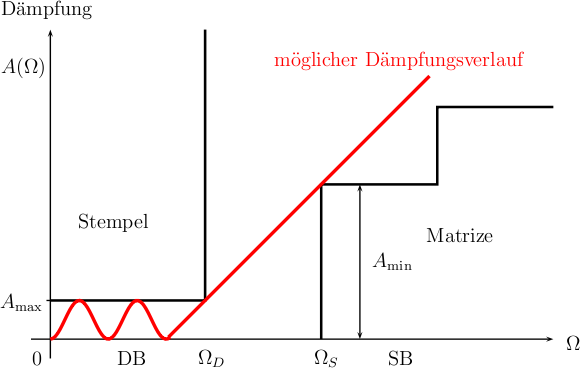
\includegraphics[width=6cm]{./images/filter-toleranzschema.png}}
\end{tabular}

\subsection{Realisation analoger Filter}
\subsubsection{Allgemeines Vorgehen}
\begin{itemize}
  \item[1.] Frequenznormierung durchführen (Kapitel \ref{frequenznormierung})
  \item[2.] Normierten Tiefpass bestimmen (Filter nach Tiefpass transformieren) (Kapitel \ref{filtertransformation})
  \item[3.] Art der Approximation wählen: Butterworth, Tschebyscheff (I, II),
  Cauer, Bessel, Gauss, \ldots (Kapitel \ref{tiefpassapprox}
  \item[4.] Bestimmung der Ordnung mit Nomogrammen \formelbuch{404}, Formeln (Kapitel \ref{ordnung}),
	\matlab{buttord, cheb1ord, cheb2ord, ellipord}
\end{itemize}
\begin{tabular}{m{9cm}|m{9cm}}
    UTF & LC-Filer \\
  \hline
    \begin{itemize}
      \item[5.] normierter TP bestimmen
      \item[6.] Werte aus Tabellen lesen\formelbuch{408ff}
      \item[7.] entnormieren
    \end{itemize} &
    \begin{itemize}
      \item[5.] L und C Werte aus Tabellen lesen\formelbuch{423ff}
      \item[6.] Werte entnormieren
    \end{itemize}
\end{tabular}


\subsubsection{Frequenznormierung \formelbuch{308}}
\label{frequenznormierung}
\begin{tabular}{ll}
\parbox{6cm}{
	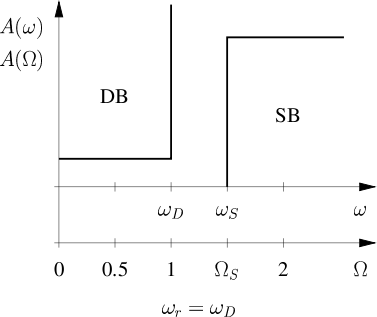
\includegraphics[width=5cm]{./images/filter-freqnormierung.png}}
& \parbox{12cm}{
	\textbf{Normierung} \\
	$\boxed{S=\frac{s}{\omega_{r}} \hspace{2cm} \Omega=\frac{\omega}{\omega_{r}} 
  \hspace{2cm} \sigma'=\frac{\sigma}{\omega_{r}}}$\\ 

	Bei BP \& BS: $\omega_r = \omega_m =\sqrt{\omega_{B1} \omega_{B2}}
	\underbrace{=}_{\text{\tiny{wenn symmetrisch}}} \sqrt{\omega_{S1} \omega_{S2}}$ \\
	
  Bei TP \& HP: $\omega_r = \omega_D$ \\

  \begin{tabular}{ll}
    $\omega_r$: & Referenzfrequenz \\
    $\omega_m$: & Mittenfrequenz
  \end{tabular} \\
  Zur Entnormierung wird $\omega_{3db}$ gebraucht, daher sind diese Formeln
	dafür nicht geeignet! \\
	}
\end{tabular}

\subsubsection{Filtertransformationen \formelbuch{355}}
\label{filtertransformation}
\renewcommand{\arraystretch}{1.5}
\begin{tabular}{|l|l|l|l|}
  \hline
  \multicolumn{2}{|l|}{\textbf{Tiefpass-Hochpass}}
    & \textbf{Tiefpass-Bandpass}
    & \textbf{Tiefpass-Bandsperre} \\ 
  \multicolumn{2}{|l|}{\parbox{6cm}{
    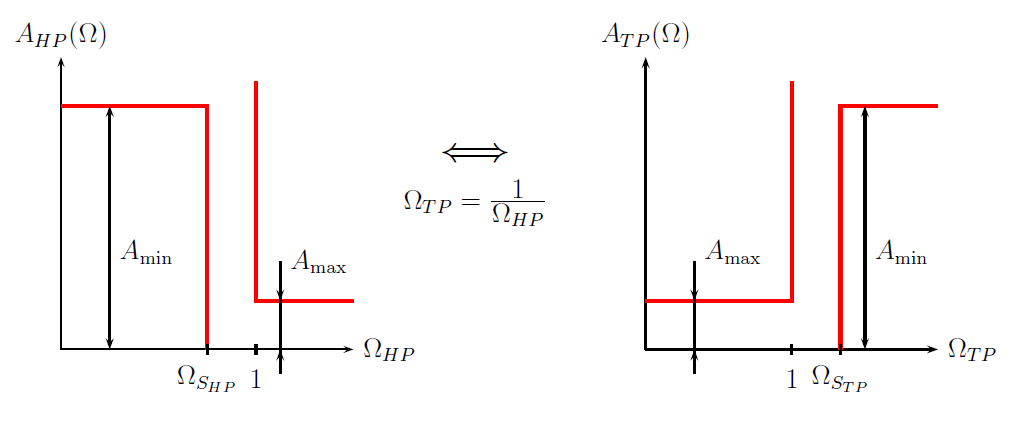
\includegraphics[width=6cm]{./images/filter-transf-tp-hp.png}
    }}
  & \parbox{6cm}{
    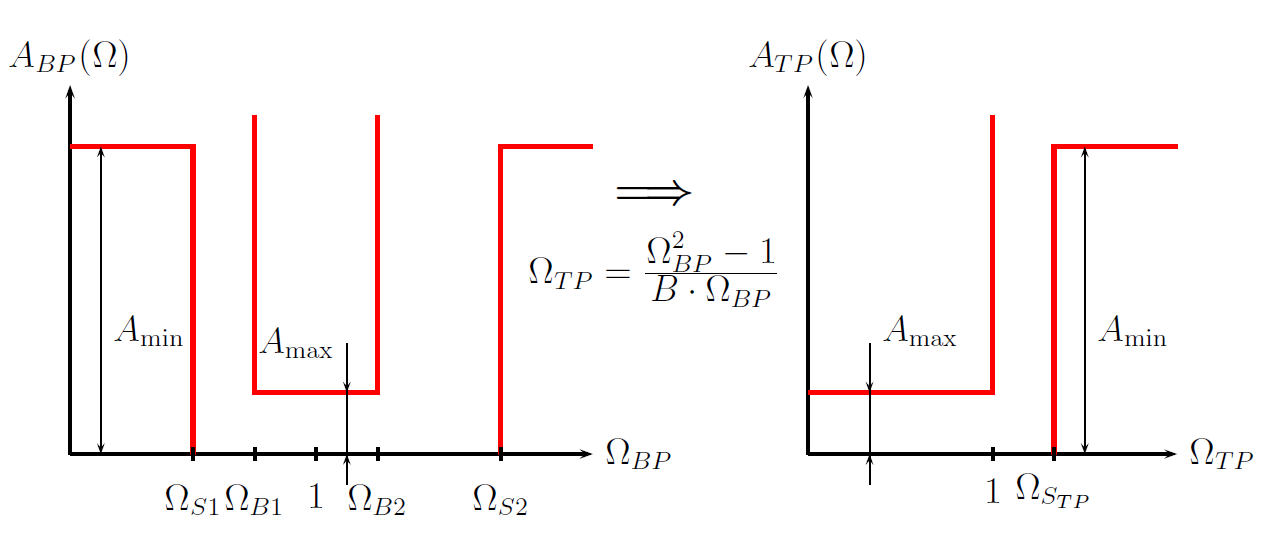
\includegraphics[width=6cm]{./images/filter-transf-tp-bp.png}
    }
  & \parbox{6cm}{
    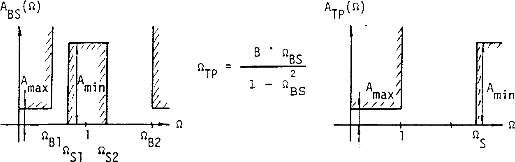
\includegraphics[width=6cm]{./images/filter-transf-tp-bs.png}
    } \\
  \hline \hline
    & \textbf{TP $\Leftrightarrow$ HP} \formelbuch{355} 
    & \textbf{TP $\Leftrightarrow$ BP} \formelbuch{360}
    & \textbf{TP $\Leftrightarrow$ BS} \formelbuch{368} \\
  \hline
  Ordnung: 
    & $n$
    & $2n$
    & $2n$ \\
  \hline
  Ansatz: 
    & $S \longrightarrow \frac{1}{S}$
    & $S \longrightarrow \frac{S^{2}+1}{B\cdot S}$
    & $S \longrightarrow \frac{B\cdot S}{S^{2}+1}$ \\
  \hline
  UTF: 
    &$H_{HP}(S)=H_{TP}\left(\frac{1}{S}\right)$
    & $H_{BP}(S)=H_{TP}\left(\frac{S^{2}+1}{B\cdot S}\right)$
    & $H_{BS}(S)=H_{TP}\left(\frac{B\cdot S}{S^{2}+1}\right)$ \\
  \hline
  Norm. Frequenz: 
    & $\Omega_{S_{TP}}=\frac{1}{\Omega_{S_{HP}}}$
    & $\Omega_{S_{TP}}=\frac{\Omega_{S2}-\Omega_{S1}}{B}=
      \frac{\Omega_{S2}-\Omega_{S1}}{\Omega_{B2}-\Omega_{B1}} =
      \frac{f_{S2}-f_{S1}}{f_{B2}-f_{B1}}$
    & $\Omega_{S_{TP}}=\frac{B}{\Omega_{S2}-\Omega_{S1}}=
      \frac{\Omega_{B2}-\Omega_{B1}}{\Omega_{S2}-\Omega_{S1}} =
      \frac{f_{B2}-f_{B1}}{f_{S2}-f_{S1}}$ \\
  \hline
  \multicolumn{2}{|l|}{normierte Bandbreite:}
    & \multicolumn{2}{|c|}{$B = \dfrac{\omega_{B2} - \omega_{B1}}{\omega_r} =
      \Omega_{B2}-\Omega_{B1}$} \\
  \hline
  \multicolumn{2}{|l|}{geometrisch-symmetrische BP/BS:}
    & \multicolumn{2}{|c|}{$\Omega_{B1}\Omega_{B2}=\Omega_{S1}\Omega_{S2}=1$}\\
  \hline
  \end{tabular}
  \renewcommand{\arraystretch}{1}
  \\
  
  \textbf{Direkte Substitution}\\
  \renewcommand{\arraystretch}{1.5}
  \begin{tabular}{|lll|}
  \hline
  HP-TP
    & $H_{TP}(S)=\frac{K}{b_{n}S^{n}+b_{n-1}S^{n-1}+...+b_{1}S+b_{0}}$
    & $\longrightarrow
    H_{HP}(S)=\frac{KS^{n}}{b_{0}S^{n}+b_{1}S^{n-1}+...+b_{n-1}S+b_{n}}$\\
  \hline
  BP-TP 1. Ordnung
    & $H_{TP}(S)=\frac{1}{S+a}$
    & $\longrightarrow 
    H_{BP}(S)=H_{TP}\left(\frac{S^{2}+1}{B\cdot S}\right)=\frac{B\cdot
    S}{S^{2}+aB\cdot S+1}$\\
  BP-TP 2. Ordnung
    & $H_{TP}(S)=\frac{1}{S^{2}+aS+b}$
    & $\longrightarrow
    H_{BP}(S)=H_{TP}\left(\frac{S^{2}+1}{B\cdot S}\right)=\frac{B^{2}S^{2}}{S^{4}+aB
    S^{3}+(bB^{2}+2)S^{2}+aB\cdot S+1}$  \\
  \hline 
  BS-TP 1. Ordnung
    & $H_{TP}(S)=\frac{1}{S+a}$
    & $\longrightarrow
    H_{BS}(S)=H_{TP}\left(\frac{B\cdot S}{S^{2}+1}\right)=
    \frac{\frac{1}{a}(S^{2}+1)}{S^{2}+\frac{B}{a}S+1}$ \\
  BS-TP 2. Ordnung
    & $H_{TP}(S)=\frac{1}{S^{2}+aS+b}$ 
    & $\longrightarrow
    H_{BS}(S) = H_{TP}\left(\frac{B\cdot S}{S^{2}+1}\right)=
    \frac{\frac{1}{b}(S^{2}+1)^{2}}{S^{4}+\frac{aB}{b}S^{3}+
    \left(\frac{B^{2}}{b}+2\right)S^{2}+\frac{aB}{b}S+1}$ \\
  \hline
\end{tabular}
\renewcommand{\arraystretch}{1}

\vfill %Füllt den Rest der Seite leer auf


\subsubsection{Tiefpassapproximationen \formelbuch{309}}
\label{tiefpassapprox}
\begin{tabular}{|p{9cm}|p{9cm}|}
\hline
\parbox[t]{9cm}{
	\textbf{Butterworth} \formelbuch{310}
	\begin{itemize}
    \item Amplitudengang: Gute Approximation (``maximal flach'', keine Welligkeit)
    \item Allpolfilter: Pole liegen auf dem Einheitskreis mit Abstand $\frac{\pi}{n}$
    \item Gruppenlaufzeit: Leichte Überhöhung bei Grenzfrequenz
    \item Bei $\Omega =1$ hat $|H(j\omega)|$ einen Abfall von 3.01dB
    \item Steilheit im SB: \qquad $-n\cdot 20dB/Dek$
	\end{itemize}
  \[ H(S) = \frac{1}{S^n +b_{n-1}S^{n-1}+\ldots+b_2S^2+b_1S+b_0}\]
	}
& 
\parbox[t]{9cm}{
	\textbf{Kritisch gedämpftes (Gauss)-Filter} \formelbuch{317}
	\begin{itemize}
    \item Keine Überschwinger bei Impuls- \& Sprungantwort
    \item Kaskadierung von wirkungsfreien identischer Filter 1.Ordnung
    \item Allpolfilter: Pole nur auf negativer $\sigma$-Achse
    \item Gruppen- und Phasenlaufzeit im DB relativ konstant
    \item Bei $\Omega = 1$ hat es eine Dämpfung 3.01dB \\
    \item Steilheit im SB: \qquad $-n\cdot 20dB/Dek$
	\end{itemize}
  \[ H(S) = \frac{K}{S^n +b_{n-1}S^{n-1}+\ldots+b_2S^2+b_1S+b_0}\]
	} \\
\hline
\parbox[t]{9cm}{
	\textbf{Tschebyscheff I} \formelbuch{321}
	\begin{itemize}
    \item Amplitudengang: Definierte Welligkeit im DB, steiler Übergang
    \item Allpolfilter, wobei alle Pole auf einer Ellipse liegen
    \item Gruppen- und Phasenlaufzeit im DB relativ konstant.
    \item Steilheit im SB: \qquad $-n\cdot 20dB/Dek$
	\end{itemize}
  \[ H(S) = \frac{K}{S^n +b_{n-1}S^{n-1}+\ldots+b_2S^2+b_1S+b_0}\]
	}
&
 \parbox[t]{9cm}{
	\textbf{Inverser Tschebyscheff  / Tscheby. II} \formelbuch{330}
	\begin{itemize}
    \item Definierte Welligkeit im Sperrbereich
    \item kein Allpolfilter
    \item Gruppen- und Phasenlaufzeit im DB relativ konstant
	\end{itemize}
	} \\
\hline
\parbox[t]{6cm}{
	\textbf{Cauer (elliptischer Filter)} \formelbuch{333}
	\begin{itemize}
    \item Amplitudengang: Definierte Welligkeit im SB und DB
    \item Steilster Übergang zwischen SB und DB
    \item bei geradem N je N konjugiert komplexe Pol- und Nullstellen
    \item bei ungeradem N 1 reeler Pol und N-1 konjugiert komplexe Pol- Nullstellen
    \item kein Allpolfilter
    \item Gruppen- und Phasenlaufzeit im DB relativ schlecht
    \item kleinste Ordnung
	\end{itemize}
	}
& 
\parbox[t]{6cm}{
	\textbf{Bessel} \formelbuch{339}
	\begin{itemize}
    \item Sehr linearer Phasengang
    \item Flachster Übergang zw. DB und SB im Amplitudengang
    \item ergibt ein Allpolfilter
    \item immer asymptotisch stabil
    \item Gruppen- und Phasenlaufzeit im DB sehr konstant
	\end{itemize}
	} \\
\hline
\end{tabular}
\vfill

\subsubsection{Bestimmung der minimal nötigen Ordnung}
\label{ordnung}
\begin{tabular}{p{7cm} p{11cm}}
\parbox{6cm}{
	\textbf{Mittels Nomogramm} \\
	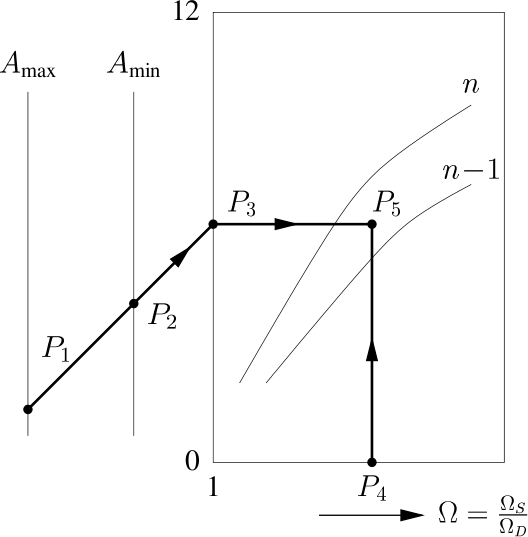
\includegraphics[width=6cm]{./images/filter-nomogramme.png}
	}
& \parbox{12cm}{
	\textbf{Oder mittels Formeln}\\
	$n_{\text{Butterworth}} \geq\frac{\log{\left[\displaystyle\frac{10^{A_{\min}/10}-1}
	{10^{A_{\max}/10}-1}\right]}} {2 \cdot \log{\left(\frac{\Omega_{S}}{\Omega_{D}}\right)}}$ \\ \\

	$n_{\text{Tschebyscheff}_{(\text{I,II})}} \geq\frac{{\rm Arcosh}\sqrt{\displaystyle\frac{10^{A_{\min}/10}-1}
	{10^{A_{\max}/10}-1}}}{{\rm Arcosh}\left({\Omega_{S}/\Omega_{D}}\right)}$ \\ \\

	$n_{\text{Cauer}} \geq\frac{K\left(\left( \frac{\Omega_D}{\Omega_S}\right)^2\right)
	K\left(1-\frac{10^{A_{\max}/10}-1}{10^{A_{\min}/10}-1}\right) } {K\left(1-\left(\frac{\Omega_D}
	{\Omega_S}\right)^2\right )K\left(\frac{10^{A_{\max}/10}-1}{10^{A_{\min}/10}-1} \right)},
	\text{mit}\quad
	K(k)=\int_0^{\frac{\pi}{2}}\frac{d\theta}{\sqrt{1-k\sin^2\theta}}$ \\ \\
	
	\textbf{Oder mit Matlab}\\
	\texttt{buttord, cheb1ord, cheb2ord, ellipord}	
	}
\end{tabular} \\ \\
\textbf{Grundsätzlich gilt (für gleiche Spezifikationen)} \quad
$n_{\text{Butterworth}}\geq n_{\text{Tschebyscheff}_{(\text{I,II})}}\geq n_{\text{Cauer}}$
\subsubsection{UTF bestimmen \& entnormieren}
Die UTF kann meist aus Tabellen herausgelesen werden und variiert je nach
Filtertyp. Die Entnormierung erfolgt durch Substitution von $S \longrightarrow
\displaystyle\frac{s}{\omega_{\text{3dB}}}$, wobei auch hier
$\omega_{\text{3dB}}$ je nach Filtertyp unterschiedlich berechnet wird.

\renewcommand{\arraystretch}{1.5}
\begin{tabular}{|p{6cm}|p{6cm}|p{6cm}|}
\hline
Butterworth \formelbuch{345}
	& Tschebyscheff I \formelbuch{349}
	& Kritisch gedämpfte Filter \formelbuch{347}\\
$\omega_{\text{3dB}}=\sqrt[2n]{\frac{1}{10^{A_{\max}/10}-1}}\cdot \omega_{D}$
	&
	$\omega_{\text{3dB}}=\cosh{\left[\left(\frac{1}{n}\right) {\rm
	Arcosh}\left(\frac{1}{e}\right)\right]} \cdot \omega_{D}$\newline
	Wobei $e = \sqrt{10^{A_{max}/10}-1}$
	& $\omega_{3\text{dB}}=\frac{\omega_D \cdot{\sqrt{2^{1/n}-1}}
	}{\sqrt{10^{\frac{A_{\text{max}}}{10\cdot n}}-1}}$ \\
\hline
Cauer \formelbuch{356}
	& Bessel \formelbuch{353}
	& \\
Keine Tabelle, \matlab{ellip, ellipap}
	& $\omega_{3\text{dB}}$ aus Abb. 7.93 \formelbuch{354}
	& \\
\hline
\end{tabular}
\renewcommand{\arraystretch}{1}


\subsubsection{LC-Tiefpass bestimmen \formelbuch{???,
420}}
\begin{tabular}{ll}
\parbox{10cm}{
	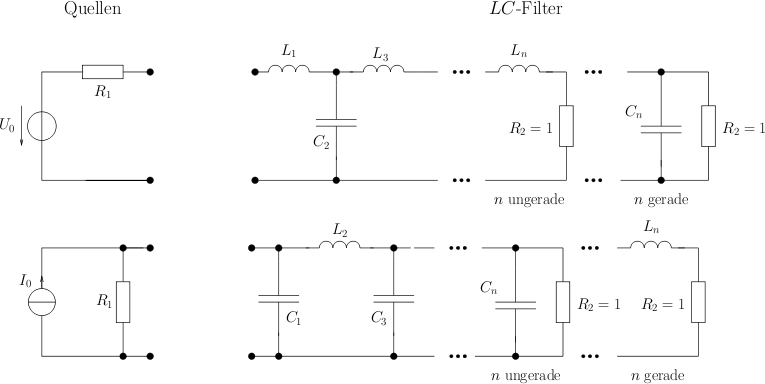
\includegraphics[width=10cm]{./images/filter-lc-realisation.png}
	}
& \parbox{8cm}{
	Die Struktur unterscheidet sich nicht zwischen den Filtertypen.\\
	Es ist zwischen Minimal-C (meistens) und Minimal-L-Netzwerken auszuwählen. \\
	\\
	Erläuterungen zu den Tabellen:
	\begin{itemize}
     \item Die Legende oben beschreibt die Stromquellenstruktur, die untere die
	Spannungsquellenstruktur.     
	\item Normierung auf $R_2 = 1$, folglich $R_1 =
	\frac{R_{\text{Quelle}}}{R_{\text{Last}}}$
    \end{itemize}
	}
\end{tabular}

\textbf{Tabellenindex} \\
\renewcommand{\arraystretch}{1.5}
\begin{tabular}{|p{5.5cm}|p{5.5cm}|p{6cm}|}
\hline
Butterworth \formelbuch{421}
	& Tschebyscheff I \formelbuch{424, 425}
	& Kritisch gedämpfte Filter \formelbuch{423}\\
\hline
Cauer \formelbuch{427, 428}
	& Bessel \formelbuch{422}
	& \\
\hline
\end{tabular}
\renewcommand{\arraystretch}{1} \\

\textbf{Entnormierung}\\
Aus den Tabellen gelesene Werte werden im folgenden als $C'$ bzw. $L'$
bezeichnet.\\ 
$C = \frac{C'}{\omega_{\text{3dB}} R_{\text{Last}}}$ \qquad $L = \frac{L'
R_{\text{Last}}}{\omega_{\text{3dB}}}$


\begin{tabular}{ll}
\parbox{11.5cm}{
	\subsubsection{Bauteiltransformation zum gewünschten Filter \formelbuch{386}}
	\renewcommand{\arraystretch}{1.5}
	\begin{tabular}{|p{2cm}|p{7.5cm}|}
	\hline
	Tiefpass-Hochpass
		& \parbox{7cm}{
		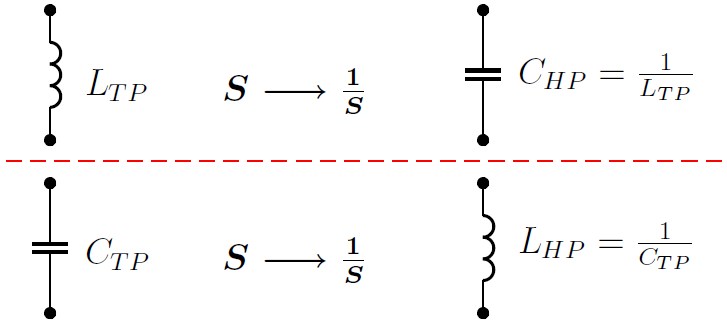
\includegraphics[width=7cm]{./images/filter-bauteile-tp-hp.png}}
		\\
	\hline
	Tiefpass-Bandpass 
		& \parbox{7cm}{
		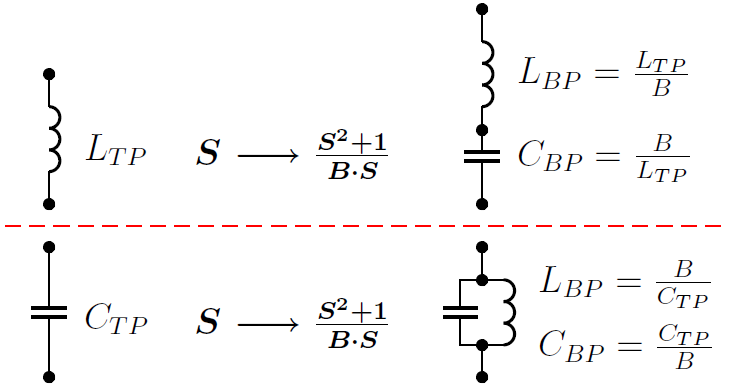
\includegraphics[width=7cm]{./images/filter-bauteile-tp-bp.png}}
		\\
	\hline
	Tiefpass-Bandsperre
		& \parbox{7cm}{
		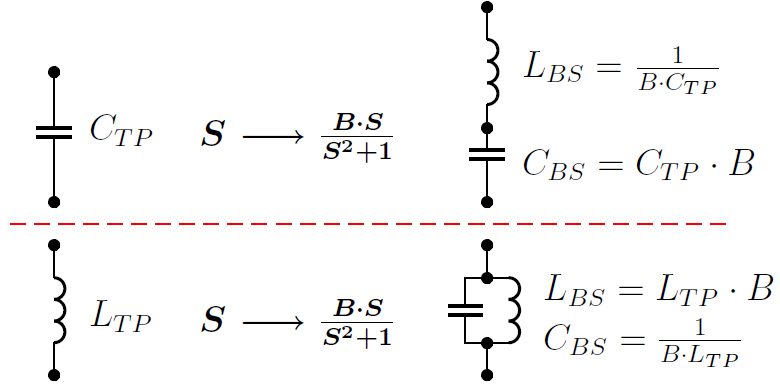
\includegraphics[width=7cm]{./images/filter-bauteile-tp-bs.png}}
		\\
	\hline
	\end{tabular}
	\renewcommand{\arraystretch}{1}
	}
& \parbox{7cm}{
	\subsection{Kaskadierung von Filtern}
	Wenn mehrere Filter kaskadiert werden, ändern sich die Spezifikationen wie in
	folgendem Beispiel:\\
	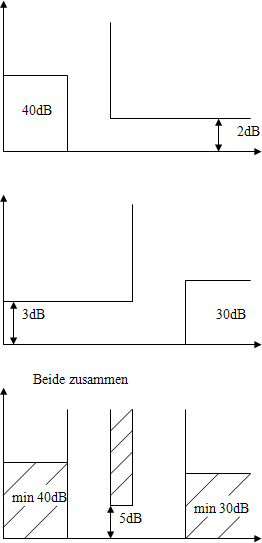
\includegraphics[width=4cm]{./images/filter-kaskadierung.png}
	}
\end{tabular}



\newpage
\subsection{Vergleich der Approximationsarten}
\scriptsize
\begin{center}
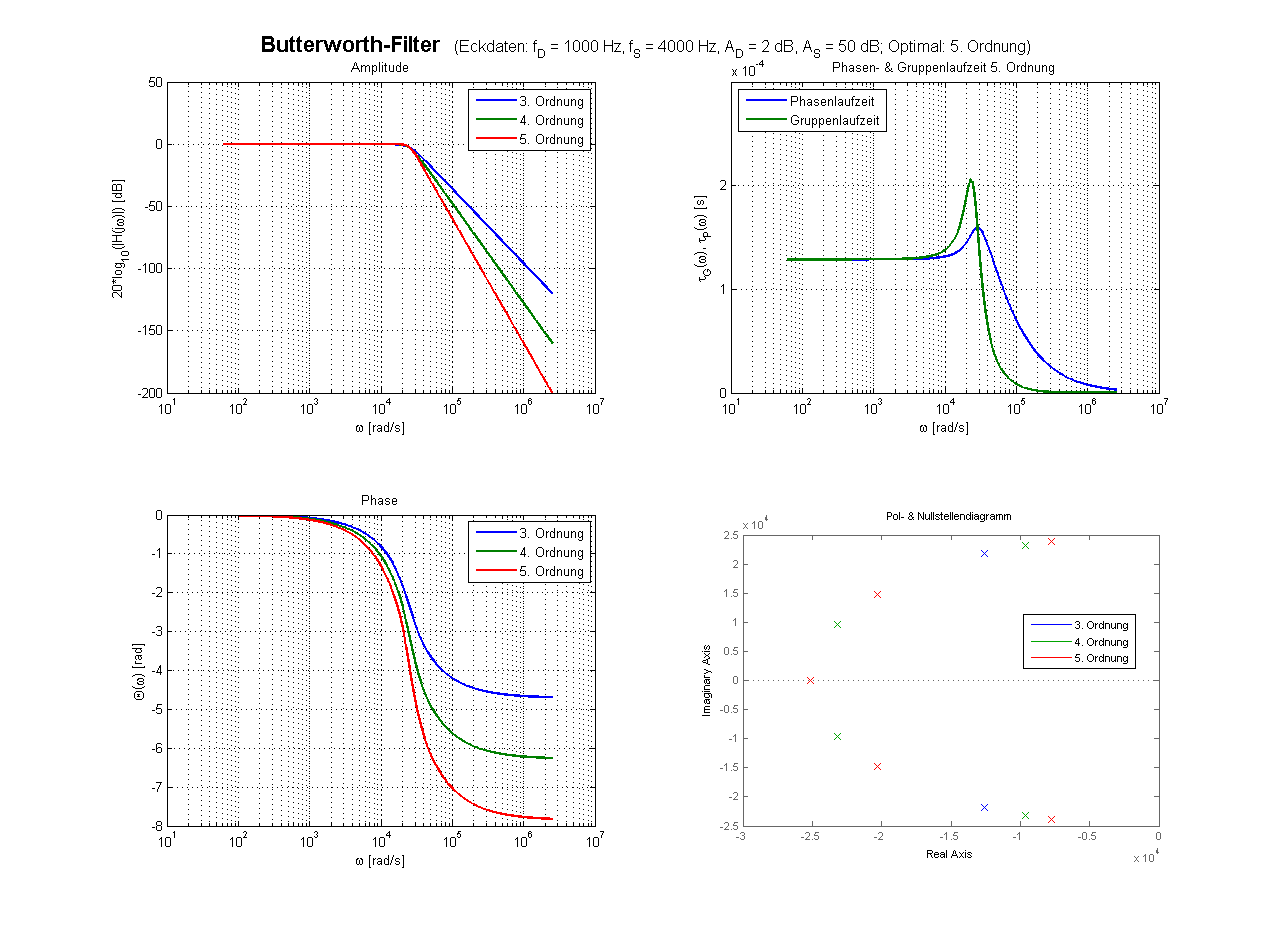
\includegraphics[height=11.5cm]{./images/filter-butterworth.png}
\\Butterworth-Filter mit UTF $H(s) = \frac{1.003e022}{s^5 + 8.133e004 s^4 +
3.307e009 s^3 + 8.312e013 s^2 + 1.291e018 s + 1.003e022}$ 
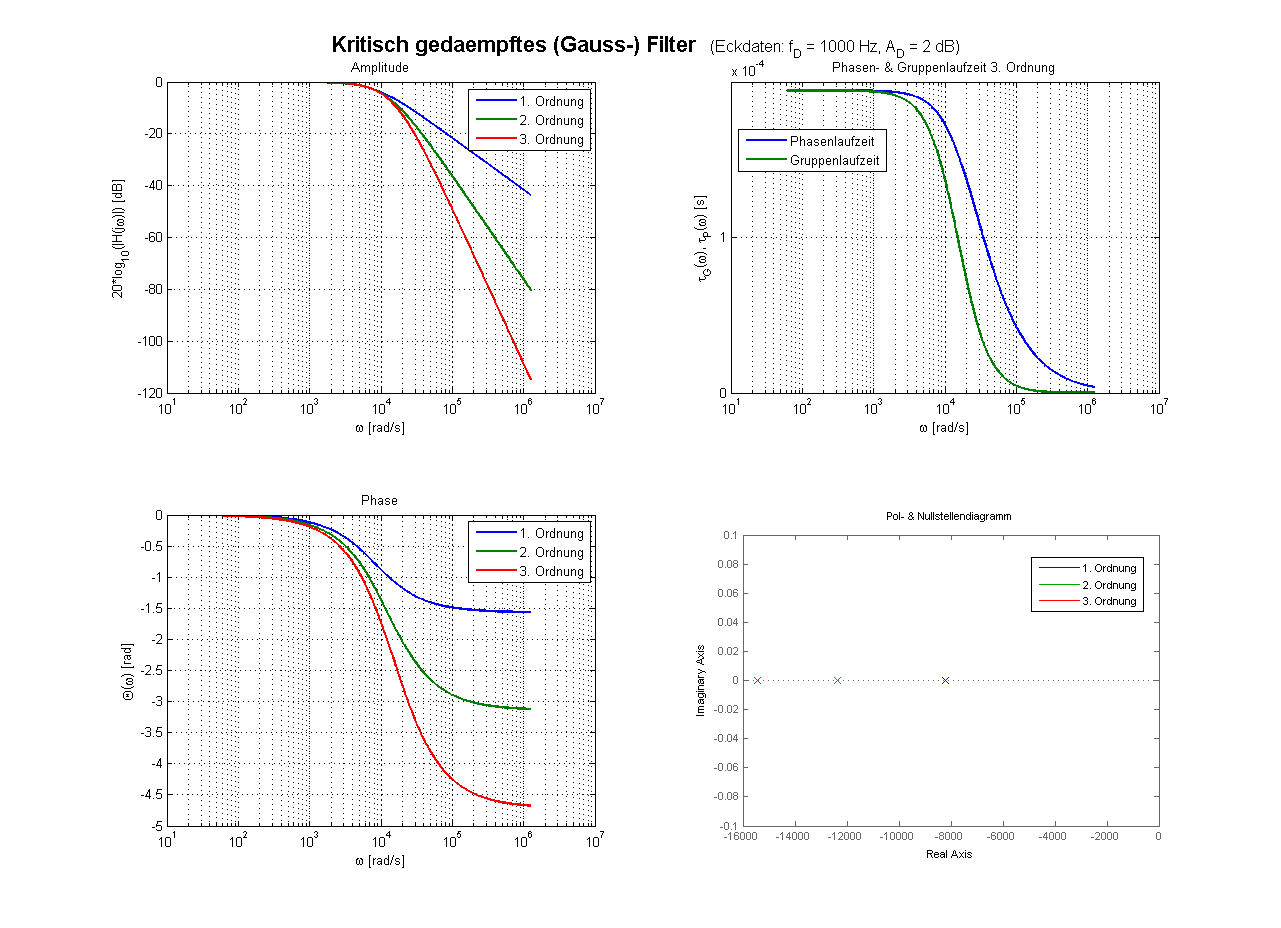
\includegraphics[height=11.5cm]{./images/filter-gauss.png} \\Kritisch gedämpftes
Filter mit UTF $H(s) = \frac{1}{2.724e-013 s^3 + 1.261e-008 s^2 + 0.0001945 s +
1}$ 
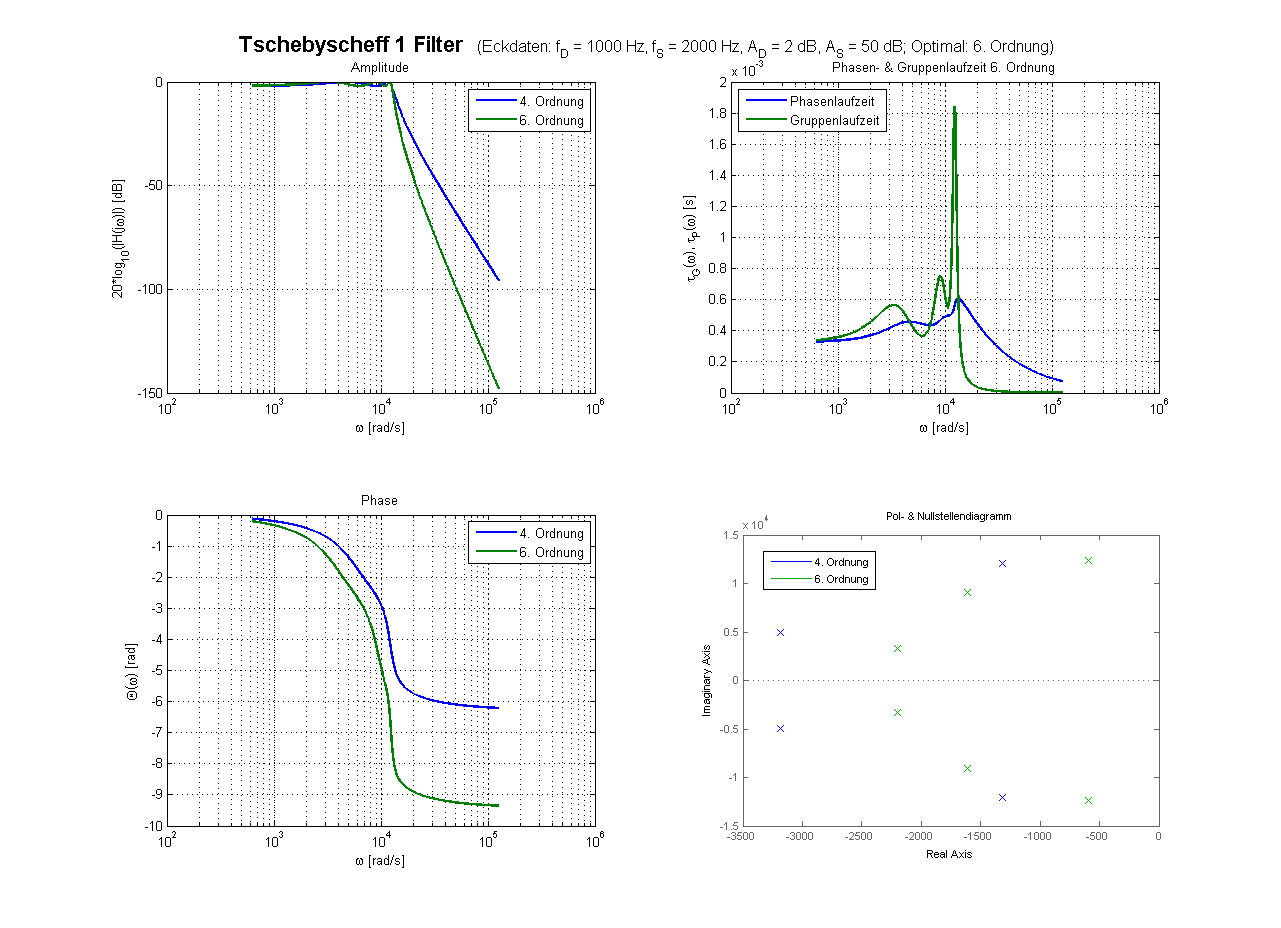
\includegraphics[height=12cm]{./images/filter-tschebyscheff1.png} \\Tschebyscheff-I-Filter mit UTF $H(s)
= \frac{1.609e023}{s^6 + 8812 s^5 + 2.757e008 s^4 + 1.721e012 s^3 + 1.924e016
s^2 + 6.589e019 s + 2.026e023}$ 
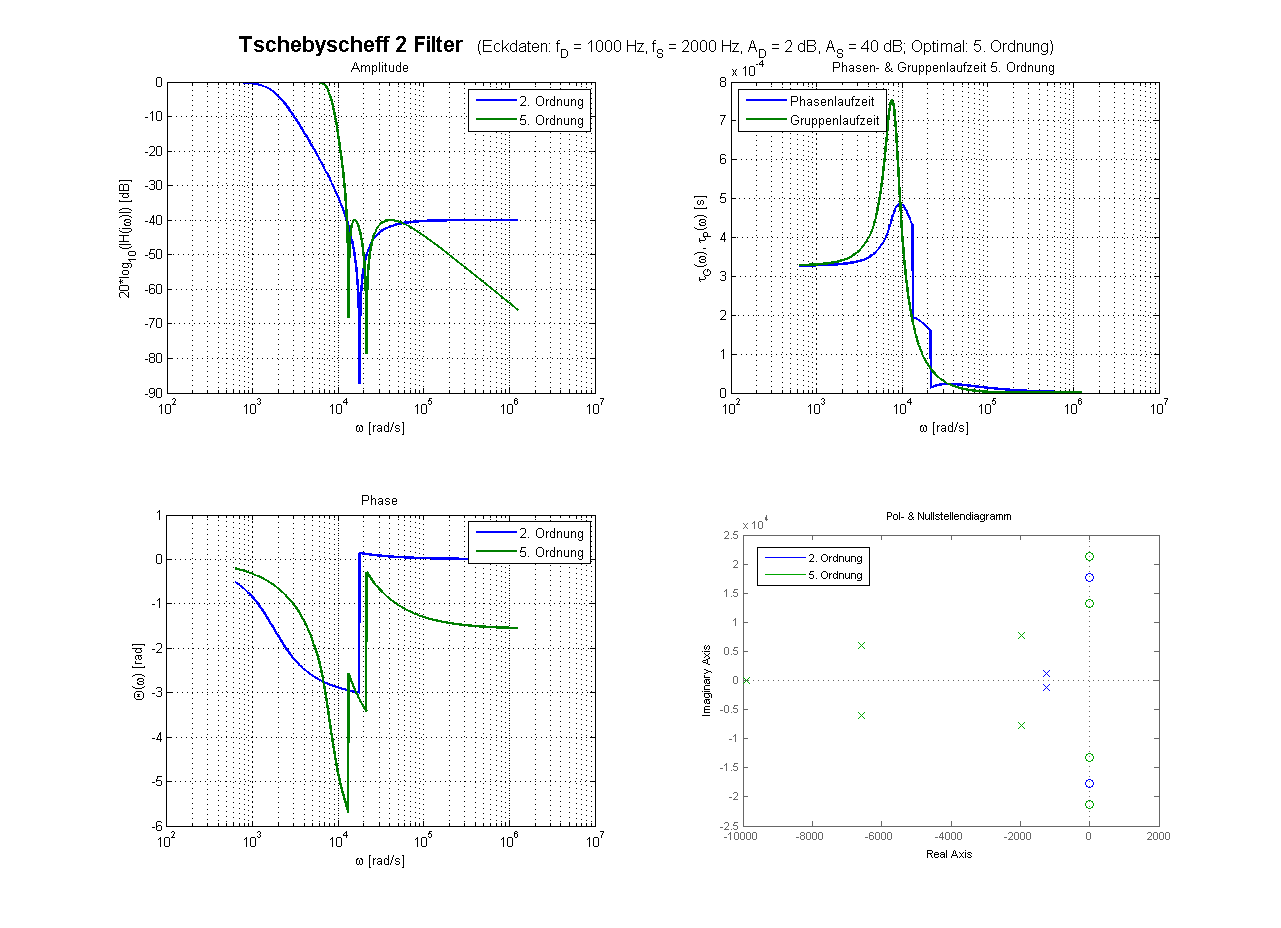
\includegraphics[height=12cm]{./images/filter-tschebyscheff2.png} \\Tschebyscheff-II-Filter mit UTF
$H(s) = \frac{628.3 s^4 + 1.081e-009 s^3 + 3.969e011 s^2 + 1.975 s +
5.014e019}{s^5 + 2.701e004 s^4 + 3.645e008 s^3 + 3.076e012 s^2 + 1.639e016 s + 5.014e019}$
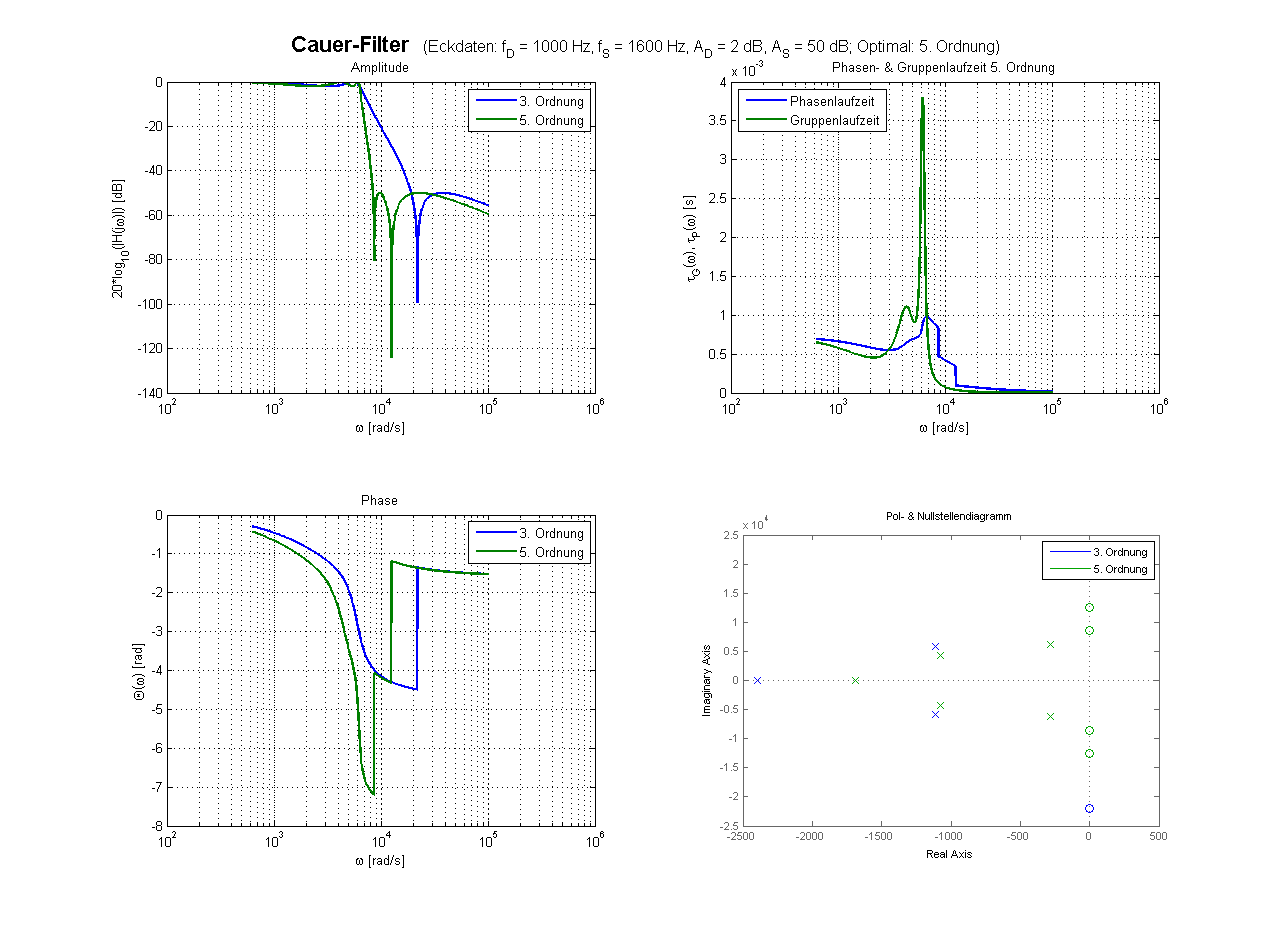
\includegraphics[height=12cm]{./images/filter-cauer.png} \\Cauer-Filter mit UTF
$H(s) = \frac{108.8 s^4 - 6.596e-010 s^3 + 2.538e010 s^2 - 0.08009 s + 1.29e018}{s^5 + 4398 s^4 + 6.408e007 s^3 + 1.939e011 s^2 + 9.227e014 s + 1.29e018}$
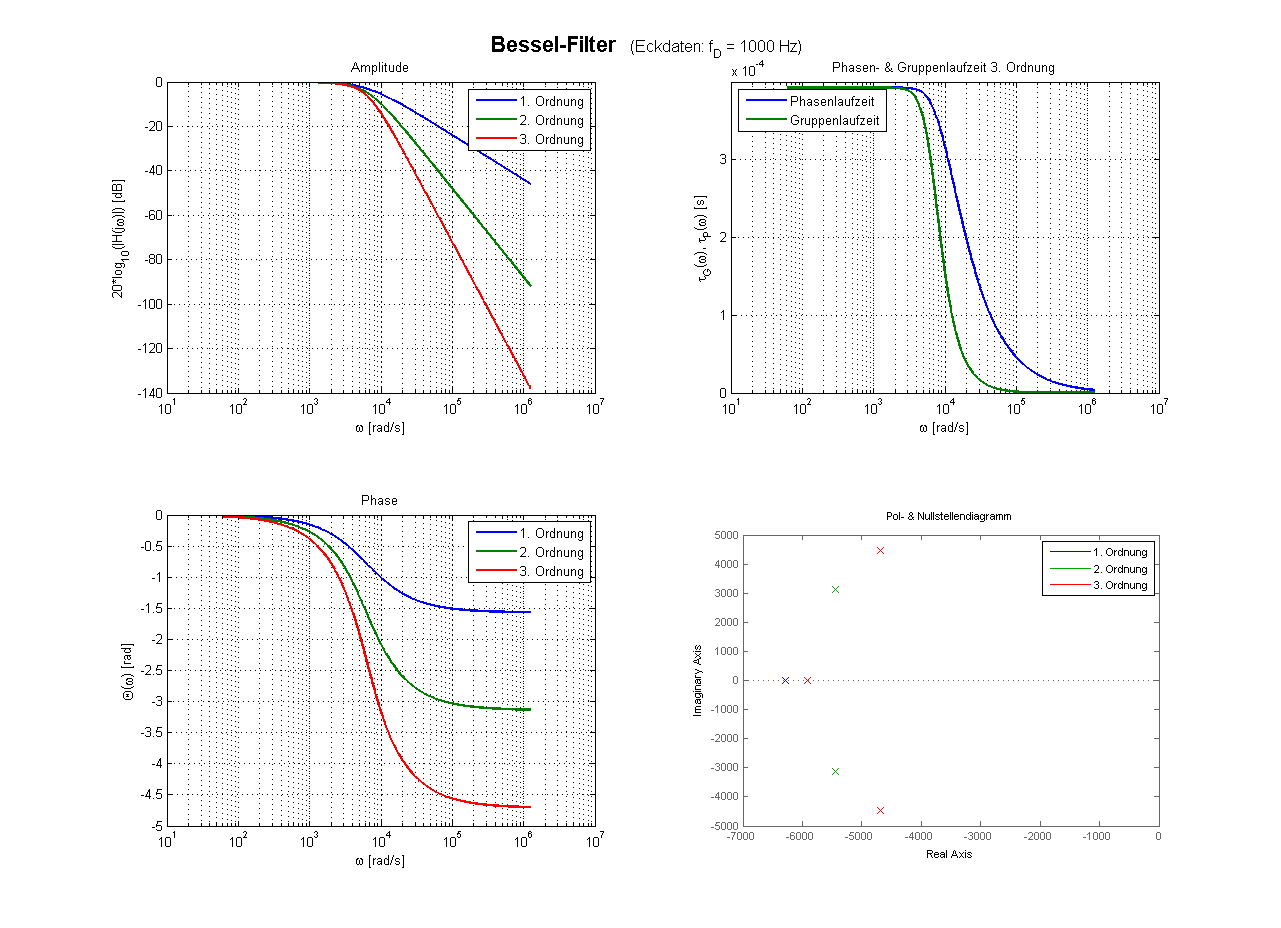
\includegraphics[height=12cm]{./images/filter-bessel.png} \\Bessel-Filter mit UTF $H(s) =
 \frac{2.481e011}{s^3 + 1.529e004 s^2 + 9.736e007 s + 2.481e011}$
\end{center}


